\documentclass{article}

\author{Jacob Thomas Errington (260636023)} \title{Assignment \#2\\Distributed
Systems -- COMP 512} \date{28 October 2015}

\usepackage{float} \usepackage{float} \usepackage{amsmath,amssymb,amsthm}
\usepackage[margin=2.0cm]{geometry}
\usepackage{algorithm,algorithmicx,algpseudocode}
\usepackage{tikz}

\usetikzlibrary{tikzmark}

\begin{document}

\maketitle

\section{Total order multicast}

Given is a group of nodes organized into clusters. Let $g_1, \cdots, g_n$
denote these clusters. Each cluster $g_i$ contains a single distinguished
process denoted $p^\prime_i$ called the control process. Now we can establish
the two kinds of communication groups in this system.

\begin{enumerate}
    \item A \emph{regular communication group} consists of all members of
        a group $g_i$. There are $i$ such groups under consideration.
    \item The \emph{control group} $g^\prime$ consists of all the control
        processes, i.e. $g^\prime = \{p^\prime_1, \cdots, p^\prime_n\}$. There
        is exactly one control group, and it has $n$ members.
\end{enumerate}

Messages are to be transmitted between all nodes in a totally ordered fashion.
To achieve this, the control process of each cluster will act as a sequencer
within its cluster, and the control group will operate using a token ring
approach. Below are the different scenarios that can arise in this scheme.

\begin{enumerate}
    \item When a regular process wants to multicast a message, it simply sends
        it to the control process of its cluster.

    \item When a control process receives a message from an ordinary process in
        its cluster, it will add it to a queue $Q$.

    \item When a regular process receives a message from its associated control
        process, it delivers it in the order given by the sequence number of
        the message.

    \item When a control process receives a message from another control
        process, it simply adds it to a queue $P$ prioritized on the sequence
        numbers of received messages. Notice that this priority queue is
        separate from the queue of cluster-local messages.

    \item When a control process receives the token from another control
        process, it multicasts its enqueued messages to each of the processes
        in its cluster and to every other control node, assigning sequence
        numbers to the messages according to the sequence number contained by
        the token.
\end{enumerate}

Of these scenarios, only the last one's implementation is nontrivial, so it is
given in full in algorithm \ref{alg:token-receive}.

\begin{algorithm}[ht]
    \caption{A control process receives the token.}
    \label{alg:token-receive}
    \begin{algorithmic}
        \Require{
            The token $t$,
            the remote message queue $P$,
            the cluster-local queue $Q$,
            the next control process ID $j$.
        }
        \Ensure{
            Messages in $Q$ are transmitted to all processes in the local
            cluster and to all other control processes, and messages in $P$ are
            delivered to all processes in the local cluster.
        }
        \State ~
        \While{$|P| > 0$}
            \State $m, seq \gets$ \Call{Dequeue}{P}
            \For{each process $p$ in the local cluster}
                \State \Call{Send}{$p$, $\left\langle m, seq\right\rangle$}
            \EndFor
        \EndWhile
        \State $n \gets t.seq$
        \While{$|Q| > 0$}
            \State $m \gets$ \Call{Dequeue}{Q}
            \For{each process $p$ in the local cluster}
                \State \Call{Send}{$p$, $\left\langle m, n\right\rangle$}
            \EndFor
            \For{each other control process $p^\prime$}
                \State \Call{Send}{$p$, $\left\langle m, n\right\rangle$}
            \EndFor
            \State $n \gets n + 1$
        \EndWhile
        \State $t.seq \gets n$
        \State \Call{SendToken}{$t$, $p_j$}
    \end{algorithmic}
\end{algorithm}

\section{Serializability and schedules}

Given are the following schedules.

\begin{align*}
    S_1 &= r_1 (a), r_2 (b), r_2 (a), w_2 (a), c_2, w_3 (c), r_1 (c), c_1, r_3 (b), c_3 \\
    S_2 &= w_1 (a), w_2 (b), r_3 (c), r_3 (a), c_3, r_1 (b), c_1, w_2 (c), c_2
\end{align*}

\begin{enumerate}
    \item
        The dependency graphs of $S_1$ and $S_2$ are given in figures
        \ref{fig:dependency-graph-s1} and \ref{fig:dependency-graph-s2},
        respectively.

        \begin{figure}[ht]
            \centering
            \begin{tikzpicture}[
                    ->,
                    shorten >=1pt,
                    auto,
                    node distance=3.0cm,
                    semithick
                ]
                \node (T1) {$T_1$};
                \node (T2) [below left of=T1] {$T_2$};
                \node (T3) [below right of=T1] {$T_3$};

                \path
                (T3) edge node {} (T1)
                (T1) edge node {} (T2)
                ;
            \end{tikzpicture}
            \caption{The dependency graph for the schedule $S_1$.}
            \label{fig:dependency-graph-s1}
        \end{figure}

        \begin{figure}[ht]
            \centering
            \begin{tikzpicture}[
                    ->,
                    shorten >=1pt,
                    auto,
                    node distance=3.0cm,
                    semithick
                ]
                \node (T1) {$T_1$};
                \node (T2) [below left of=T1] {$T_2$};
                \node (T3) [below right of=T1] {$T_3$};

                \path
                (T1) edge node {} (T3)
                (T3) edge node {} (T2)
                (T2) edge node {} (T1)
                ;
            \end{tikzpicture}
            \caption{The dependency graph for the schedule $S_2$.}
            \label{fig:dependency-graph-s2}
        \end{figure}

        The schedule $S_1$ is serializable. There is one equivalent serial
        schedule.

        \begin{center}
            \begin{tabular}{c | c | c}
                &      & w(c) \\
                &      & r(b) \\
                &      & c \\
                r(a) &      & \\
                r(c) &      & \\
                c    &      & \\
                     & r(b) & \\
                     & r(a) & \\
                     & w(a) & \\
                     & c    &
            \end{tabular}
        \end{center}

        The schedule $S_2$ is not serializable. Here are the conflicting
        operations.

        \begin{align*}
            r_3 (a) &\to w_1 (a) \\
            r_1 (b) &\to w_2 (b) \\
            r_3 (c) &\to w_2 (c)
        \end{align*}
\end{enumerate}

\section{Serializability}

Given is a transaction management algorithm.

We will first analyze the different transaction anomalies that can occur in
this system.

\begin{enumerate}
    \item
        Lost updates are not possible in the given transaction management
        algorithm.  All values to write are stored in the WriteSet.
        Furthermore, each entry in the WriteSet has a corresponding entry in
        the ReadSet. The corresponding ReadSet entry for each WriteSet entry to
        be written is compared with its value in the backing store, in order to
        check for potentially overwriting an update made by a concurrent
        transaction. This mitigates the possibility of lost updates.

        The \emph{closeTransaction} function is responsible for verifying that
        the data held by the backing store is the same as when it was first
        read.

    \item
        Unrepeatable reads are not possible in this scheme either. When read
        requests are submitted in the transaction, the transaction manager will
        check in the WriteSet and then in the ReadSet for the value before
        loading it from the backing store. Hence, one transaction cannot alter
        another transaction's ``view'' of the data.

        The \emph{read} function's if-statements, checking whether the data
        item to read has already been read or written (and hence ``cached''
        within the transaction) prevents the unrepeatable read anomaly from
        occcurring.

    \item
        Write skew is possible in this scheme. Suppose that we have a
        constraint that the sum of the data items $a$ and $b$ be at least zero.
        Two transactions might independently alter the values of $a$ and $b$
        respectively, thinking that the constraint is satisfied, but the
        overall outcome of the two transactions might leave the data in an
        undesirable state.

        The \emph{closeTransaction} function in particular is what allows this
        anomaly to occur, as it does not check that constraints are still
        satisfied.

    \item
        Dirty reads are impossible in this system. Only committed data is read
        because the transactions operate on local copies of the data in
        volatile memory when they perform updates and only persist their data
        to the backing store upon committing the transaction. Hence,
        uncommitted data from another transaction cannot be read. Of course, a
        transaction will read its own uncommitted writes, but that is expected
        behaviour.

        The \emph{read} function is what guarantees that the local copy of the
        data item is read rather than the value currently in the backin store,
        and the \emph{closeTransaction} function is what guarantees that data
        is persisted only when the transaction complete, mitigating the
        possibility of a concurrent transaction retrieving uncommitted data.

    \item
        Dirty writes are impossible in this system. Since uncommitted data is
        never persisted to the backing store, writing data to the backing store
        cannot result in the overwriting of an uncommitted value. Furthermore,
        since exclusive locks are acquired prior to the writing to the backing
        store, the possibility of interleaved writes is mitigated.

        These guarantees come from the implementation of the \emph{write}
        function, which records updates to the WriteSet in volatile memory
        rather than directly to the backing store. The data in the WriteSet is
        then persisted to the backing store only upon committing the
        transaction with the \emph{closeTransaction} function, which does so
        using exclusive locks so as to prevent undesirable interleaving of
        commits.
\end{enumerate}

Now we consider a schedule that this concurrency mechanism will permit, but
that is not serializable. The schedule that we will present will furthermore
not contain any lost update, unrepeatable read, or write skew anomalies.

To build this schedule, we will make use of the fact that upon committing the
transaction, the given concurrency mechanism merely checks for equality. In
particular, suppose a long-running transaction $T_1$ reads a data item $x = a$.
Meanwhile, a transaction $T_2$ sets the value of $x$ to $b$ and commits. Then,
another transaction $T_3$ sets the value of $a$ back to $a$. Finally, $T_1$
commits. Strictly speaking, this results in a dependency cycle even though the
outcome looks like there isn't one.

Concretely, here is such a problematic schedule.

\begin{center}
    \begin{tabular}{ l | l | l }
        Transaction 1          & Transaction 2                 & Transaction 3                \\ \hline
        beginTransaction       & beginTransaction              & beginTransaction             \\
        read(a)\tikzmark{t11}  &                               &                              \\
                               & read($a$)\tikzmark{t21}       &                              \\
                               & \tikzmark{t22} write($a + 5$) &                              \\
                               & closeTransaction              &                              \\
                               &                               & \tikzmark{t31}read(a)        \\
                               &                               & \tikzmark{t32}write($a - 5$) \\
                               &                               & closeTransaction             \\
        write(a)\tikzmark{t12} &                               &                              \\
        closeTransaction       &                               &                              \\
    \end{tabular}
\end{center}

\begin{tikzpicture}[
        remember picture,
        overlay,
        -latex,
        blue!75,
        shorten >=1pt,
        shorten <=1pt
    ]
    \path
    ({pic cs:t11}) edge                node {} ({pic cs:t22})
    ({pic cs:t21}) edge [bend left=30] node {} ({pic cs:t31})
    ({pic cs:t32}) edge                node {} ({pic cs:t12})
    ;
\end{tikzpicture}

The arrows overlayed on the table show the conflicting operations, and in turn
show the form of the dependency graph of the transactions.

\section{Location of lock manager}

\end{document}
